\documentclass[letterpaper]{article}%
\input{tex-util/misc.tex}
\input{tex-util/figures.tex}
\input{tex-util/homeworks.tex}
\input{tex-util/listings.tex}
\input{tex-util/math.tex}
\usepackage[letterpaper]{geometry}%
\usepackage{fancyhdr}%
\usepackage{titlesec}%

\geometry{%
  top=2.5cm,
  inner=2.5cm,
  outer=2.5cm,
  bottom=2.5cm,
  headheight=3ex,
  headsep=2ex
}
\pagestyle{fancy}
\usepackage{hyperref}

\def\CourseTitle{Advanced Database Systems}
\def\CourseNumber{CSCI-GA.2434-001}
\def\Instructor{Prof. Dennis Shasha}
\def\HomeworkSetNumber{2}

\author{%
  Brandon Reiss \& Kevin Mullin
}

\date{Tuesday, November 19th, 2013}
\title{%
  \CourseTitle{} - Homework \HomeworkSetNumber{} \\
  {\large \Instructor{}} \\
  {\large \CourseNumber{}}
}

\lhead{\CourseNumber{} - Problem Set \HomeworkSetNumber{}}
\chead{}
\rhead{Reiss \& Mullin, \thepage{} of \pageref{LastPage}}
\fancyfoot{}

\parindent0pt \parskip8pt % make block paragraphs

\begin{document}
\noindent
\maketitle
\thispagestyle{empty}

\begin{problemcopy}
ReserveWithUs is an electronic portal for hotel rooms. It buys rooms at
discounted rates and sells them for a bit more (see hotels.com for a real-life
model of such a company). The company is composed of a purchasing department
that negotiates deals with hotels and a sales department that monitors customer
activities. Each hotel has a few types of room (e.g., superior, king, queen).
For each type of room in a given hotel, the purchasing department negotiates a
block of rooms of a given type at a given price on a given day. Potential
customers browse the web site to find attractive hotels and room deals.
Possibly, they log in and add a (number of) rooms to their shopping cart.
Customers can then buy all the rooms in their shopping cart, a so-called
shopping cart checkout, where the information about the booked rooms are
committed to the database and archived. You are the IT person at ReserveWithUs
and you have been given a simple application server. The application server is
written in Java (tested on Java 1.6). The application server together with the
database schema and scripts to generate data is available at
http://code.google.com/p/databasetuning-cases/. The design of the application
server is described on that web site. The source code is available and you
should take some time to familiarize yourself with it.

Your job is to tune the database portion of the application in your environment
and to redesign some portions of the application server that are poorly
designed. Specifically, your project is to document the following tasks (back
up your claims with arguments where possible with quantitative arguments based
on experiments):
\end{problemcopy}

\def\RWUApp{\texttt{ReserveWithUsApp}}

\section{Introduction}

All code artifacts, notes, and data for this project are available online at \\
\url{https://github.com/blr246/adbs-reservewithus}.

\subsection{Environment Setup}

Configuration of the DB2 and \RWUApp{} environments involves several non-trivial
steps. Here we outline them briefly.
\vspace{1em}

\textbf{The following are software requirements needed to establish the database
environment:}
\begin{itemize} \itemsep -0.25em
  \item VirtualBox 4.3.2
  \item Ubuntu Server Edition 12.04 LTS
  \item IBM DB2 Server 10.5
  \item Apache Maven 3.0.5
  \item OpenSSH 5.6
  \item Python 2.7
\end{itemize}
\vspace{1em}

\textbf{The sequence of required steps is as follows.}
\begin{enumerate}
  \item Create a VirtualBox VM and install Ubuntu Server Edition 12.04 LTS

  \item Install IBM DB2 Server 10.5
    \begin{Verbatim}[frame=single]
# CONNECTING TO THE VM
# --------------------
# Setup Port Forwarding rule tcp,,2222,,22
# Access the VM via ssh:
$ ssh -p 2222 db2@localhost
# An X tunnel is required for GUI DB2 install:
$ ssh -p -X 2222 db2@localhost

# COMMANDS TO RUN ON THE VM
# -------------------------
$ sudo apt-get install libaio1 ksh libstdc++6-4.4-dev libstdc++6-4.4-pic
$ sudo libstdc++5 rpm apt-get install libxft libxft2 libxtst6 libxi6 libnuma1
$ wget https://www6.software.ibm.com/sdfdl/v2/regs2/db2pmopn/db2_v105/expc/Xa.2/
Xb.aA_60_-idUY9yzWtWuXp2IZA3QKPFeQlUnmFkowTtw/Xc.db2_v105/expc/v10.5fp1_linuxx64
_expc.tar.gz/Xd./Xf.LPr.D1vk/Xg.7281828/Xi.swg-db2expressc/XY.regsrvs/XZ.Vi6sUFq
Hh9kK69b7hx6M7FHeXrs/v10.5fp1_linuxx64_expc.tar.gz
$ tar -zxvf v10.5fp1_linuxx64_expc.tar.gz
$ cd expc/db2/linuxamd64/install
# Perform a root installation to allow multiple instances.
$ sudo ./db2setup
# Setup default instance, fenced user
# Setup Port Forwarding rule tcp,,2121,,5001
    \end{Verbatim}

    After the DB2 installation completes, we have a single DB2 instance with a
    database called \texttt{tuning}. The instructions posted at
    \url{https://code.google.com/p/databasetuning-cases/wiki/ReserveWithUs}
    explain how to load data into the database.

  \item Setup and configure the application server program from
    \texttt{ReserveWithUs-2.3.zip}. The original project package contains
    project files for the Netbeans Java IDE. These files do not provide a
    sufficient java environment needed to package and deploy the \RWUApp{} jar.

    To workaround this issue, the \RWUApp{} project was converted to an Apache
    Maven project mainly by reorganizing the source tree and adding a
    \href{%
      https://github.com/blr246/adbs-reservewithus/blob/master/ReserveWithUsApp/pom.xml%
    }{\texttt{pom.xml}}
    file. In addition, a special installation script called
    \href{%
      https://github.com/blr246/adbs-reservewithus/blob/master/ReserveWithUsApp/m2-install-db2jcc.sh%
    }{\texttt{m2-install-db2jcc.sh}} was created in order to install a local
    repository for the DB2Jcc Java DB2 Driver. After conversion to Maven, the
    project may be built and run in two simple steps:
    \begin{Verbatim}[frame=lines]
$ mvn package
$ java -jar target/ReserveWithUsApp-1.0.jar
    \end{Verbatim}

    The full Maven conversion is available
    \href{%
      https://github.com/blr246/adbs-reservewithus/commit/%
      fd68b867a8dd5a7cb88058cf4a24ca59dd8575eb%
    }{here}.
\end{enumerate}

\section{Tuning}

Tuning is the set of activities required to optimize frequently used queries or
to remove bottlenecks from the database system. The following sections describe
how we achieve performance gains for essential ReserveWithUs features.

\subsection{Benchmarking}

Prior to tuning, we developed a proper benchmark procedure in order to
establish a baseline and to track performance gains. One important decision was
whether to benchmark using the application interface or directly on the DB2
server. Ultimately we decided to use the application interface in order to
avoid bugs caused by failure to reproduce the proper query syntax. The
benchmark tool captures distributions of query response times using randomly
generated queries.

\subsubsection{Query distributions}

In order to generate a set of queries randomly for testing we first exported
from the database the count distributions of \texttt{(CITY, COUNTRY)} and
\texttt{(SINGLE\_ROOM\_DAY)} tuples from the \texttt{HOTEL} and
\texttt{ROOM\_DATE} tables, respectively. The data in
Table~\ref{tab:benchmarktools} describe the relevant files. Random queries are
useful because they increase the likelihood that we will see major anomalies in
performance during testing, and they are more likely to strain the database
system by playing an adversary to its caches.

\begin{table}[h]
  \centering
  \begin{tabular}{ll}
    \toprule
    filename & description \\
    \midrule
    \href{%
      https://github.com/blr246/adbs-reservewithus/blob/master/ReserveWithUsDB/query_data_commands.sh%
    }{\texttt{query\_data\_commands.sh}} & collects data distributions needed for benchmarking \\
    \href{%
      https://raw.github.com/blr246/adbs-reservewithus/master/ReserveWithUsApp/query_data/country_city_counts.csv%
    }{\texttt{country\_city\_counts.csv}} & data file for \texttt{(CITY, COUNTRY)} tuples \\
    \href{%
      https://raw.github.com/blr246/adbs-reservewithus/master/ReserveWithUsApp/query_data/date_counts.csv%
    }{\texttt{date\_counts.csv}} & data file for \texttt{(SINGLE\_ROOM\_DAY)} tuples \\
      \href{%
      https://github.com/blr246/adbs-reservewithus/blob/master/ReserveWithUsApp/benchmark_queries.py%
    }{\texttt{benchmark\_queries.py}} & benchmarking tools \\
    \bottomrule
  \end{tabular}
  \caption{Files associated with DB2 benchmarking.}
  \label{tab:benchmarktools}
\end{table}

During benchmark execution, the \texttt{(CITY, COUNTRY)} tuples are sampled in
a random uniform fashion such that if a particular tuple appeared in 50\% of
the hotel inventory, then it would be 50\% likely to be selected for a query.
Date intervals are selected by using a log-normal distribution in order to
favor shorter date ranges. This matches the intuition that people more
generally purchase shorter stays at hotels with a long tail toward durations
over a couple of weeks. A better model for query generation would be to use
actual customer queries played back from server logs, but such data are not
available.

\subsubsection{Running benckmarks}

Benchmarks are executed using the \texttt{iPython} REPL. The advantage over a
command-line application is more rapid prototyping. The following code listing
shows an example usage of the benchmark tool.

\begin{Verbatim}[frame=single]
$ ipython
In [1]: import numpy as np
In [2]: import benchmark_queries as bq
In [3]: times = bq.mode_test_i_hotels('target/ReserveWithUsApp-1.0.jar', 100)
select h.hotel_id, h.name, h.street, h.city, h.zip_code, h.state, h.country, h.r
ating, h.distance_to_center from hotel h where h.city = 'city201' and h.country 
= 'country14'
command=search_hotels&country=country14&city=city201
hotel command 1 of 100: time=0.016166s, len(result)=6
select h.hotel_id, h.name, h.street, h.city, h.zip_code, h.state, h.country, h.r
ating, h.distance_to_center from hotel h where h.city = 'city137' and h.country 
= 'country3'
command=search_hotels&country=country3&city=city137
hotel command 2 of 100: time=0.018512s, len(result)=9
...
...
select h.hotel_id, h.name, h.street, h.city, h.zip_code, h.state, h.country, h.r
ating, h.distance_to_center from hotel h where h.city = 'city141' and h.country 
= 'country2'
command=search_hotels&country=country2&city=city141
hotel command 99 of 100: time=0.016742s, len(result)=9
select h.hotel_id, h.name, h.street, h.city, h.zip_code, h.state, h.country, h.r
ating, h.distance_to_center from hotel h where h.city = 'city6' and h.country = 
'country8'
command=search_hotels&country=country8&city=city6
hotel command 100 of 100: time=0.019718s, len(result)=10

In [4]: np.histogram(times)
Out[5]:
(array([ 7, 50, 34,  8,  0,  0,  0,  0,  0,  1]),
 array([ 0.01152301,  0.0139266 ,  0.01633019,  0.01873379,  0.02113738,
       0.02354097,  0.02594457,  0.02834816,  0.03075175,  0.03315535,
       0.03555894]))
\end{Verbatim}

The benchmark \texttt{mode} methods are designed to test either hotel or room
queries. The return value is a list of times. The benchmark tool is also
designed to open its own connection to the database$^*$. The \texttt{histogram}
tool is an excellent way to infer some statistics about the data collected. In
this example, the median query time is between 14.0ms and 16.4ms.

\vspace{1em}
{\small
\textsl{$^*$There is a known issue on MacOS preventing the benchmark tool from
starting its own instance of the application server.  A valid workaround is to
start the application server in another terminal prior to using the benchmark
tool.}
}

\subsubsection{Test hardware}

The test hardware is listed in Table~\ref{tab:testhardware}.

\begin{table}[h]
  \centering
  \small
  \begin{tabular}{rl}
    \toprule
    component & description \\
    \midrule
    cpu & AMD Dual-Core 1.60 GHz E-350 Processor \\
    memory & 4GB DDR3 RAM \\
    disk & Seagate Momentus ST9500420AS 500GB 7200RPM SATA Disk \\
    \bottomrule
  \end{tabular}
  \caption{Test hardware configuration.}
  \label{tab:testhardware}
\end{table}

The DB2 configuration is listed in Table~\ref{tab:db2setup}.

\begin{table}[h]
  \centering
  \small
  \begin{tabular}{rl}
    \toprule
    component & description \\
    \midrule
    os & Ubuntu Server 12.04 LTS 64-bit Running on VirtualBox 4.2.18 \\
    storage & 8.00 GB Fixed Virtual Disk \\
    memory & 1296MB Physical RAM \\
    cpu & Physical CPU w/100\% Physical Exectuion Cap \\
    networking & Local NAT-based Networking \\
    db2 version & IBM DB2/LINUXX8664 10.5.1 Database Server \\
    \bottomrule
  \end{tabular}
  \caption{DB2 virtual machine configuration.}
  \label{tab:db2setup}
\end{table}

\subsection{Query on hotel and room based on country and city}

To begin, we collect a baseline set of timings for the hotel and room queries
using the benchmarking script. These plots are both visible under the title
``NO OPTIMIZATION'' in Figure~\ref{fig:hotelqueries} for hotel queries and
Figure~\ref{fig:roomqueries} for room queries. Immediately from this baseline
it is clear that the room query is the bottleneck. On the dated hardware used
for testing, the median response time for hotel queries is approximately 250ms
while median response time for room queries is approximately 4.57s with some
queries taking over 20s.

\subsubsection{Optimizing the hotel table}

\begin{figure}[h!]
  \centering
  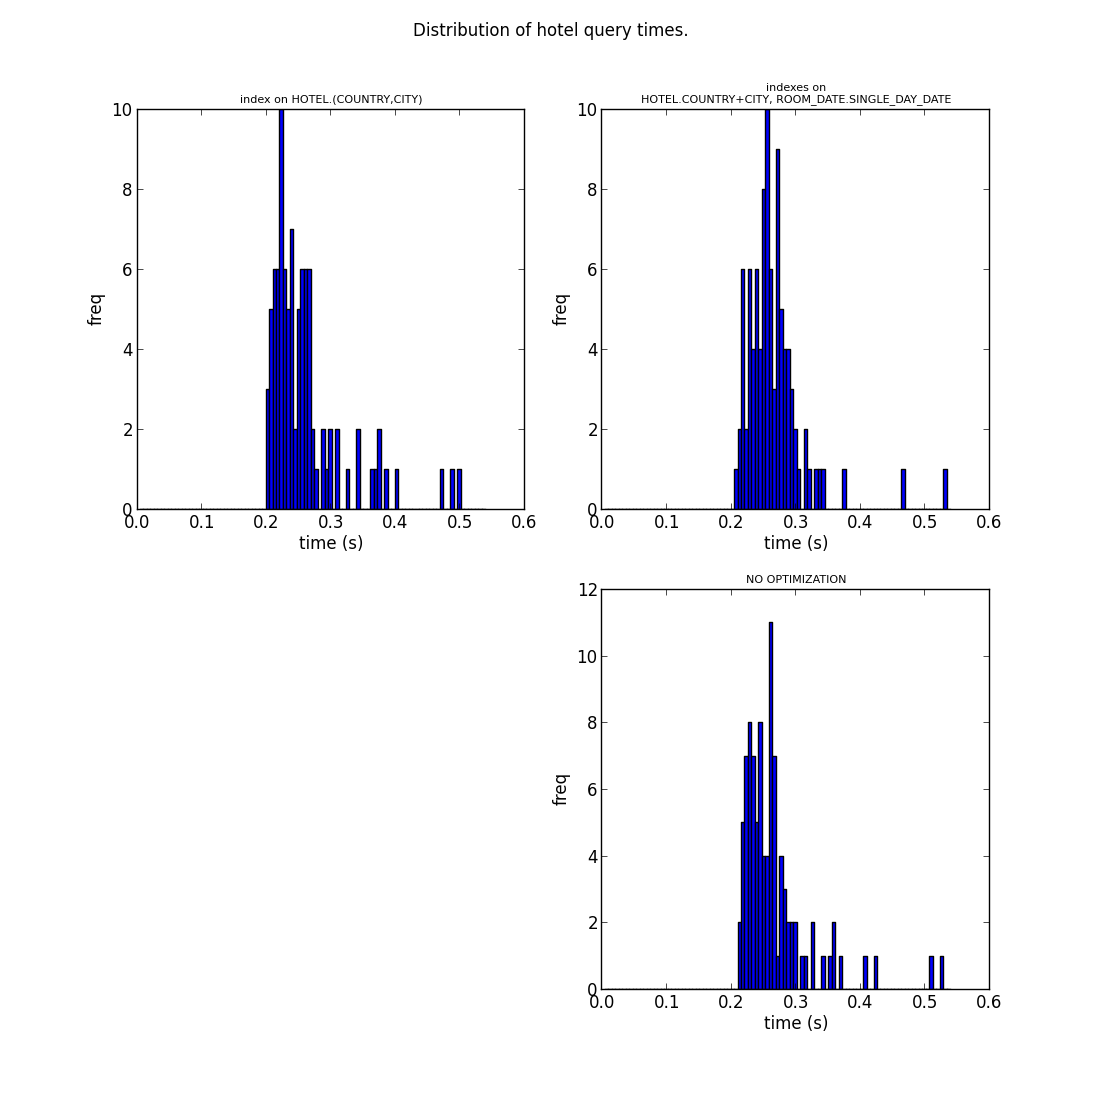
\includegraphics[width=0.66\textwidth]{../ReserveWithUsApp/benchmark_data/0.png}
  \caption{Distribution of hotel query response times. Each plot corresponds to
    performance data collected after applying some subset of the proposed
    optimizations.}
  \label{fig:hotelqueries}
\end{figure}

The customer has specified that queries on hotel by \texttt{(CITY, COUNTRY)}
are the most frequent. Assuming that ReserveWithUs is reasonably mature as a
company, we would expect a slowing down in the rate of growth for the hotel
database since the sales team will have fewer and fewer new vendors to target
for purchasing inventory. A table whose updates are infrequent and controlled
by an internal batch process is suited for the addition of a clustered index.

To make queries on \texttt{(CITY, COUNTRY)} fast, we want to arrange
sequentially on disk all hotel records for hotels having the same
\texttt{(CITY, COUNTRY)}. Traversal of the index should be very fast since
since there are only 7216 unique \texttt{(CITY, COUNTRY)} pairs and index data
structures tend to favor a large fanout.

We create the index by running the following commands:
\begin{Verbatim}[frame=single]
$ db2 CREATE INDEX HOTEL_BY_CITY_COUNTRY ON HOTEL (COUNTRY, CITY) CLUSTER PCTFRE
E 10 COLLECT DETAILED STATISTICS
DB20000I  The SQL command completed successfully.
$ db2 REORG TABLE HOTEL INDEX HOTEL_BY_CITY_COUNTRY ALLOW NO ACCESS INDEXSCAN
DB20000I  The REORG command completed successfully.
$ db2 RUNSTATS ON TABLE HOTEL AND DETAILED INDEXES ALL
DB20000I  The RUNSTATS command completed successfully.
\end{Verbatim}
The \texttt{REORG TABLE} command is used to force DB2 to reorder physically the
data on disk. The \texttt{RUNSTATS} command updates the query optimizer so that
it may use the new index. We can confirm the reorganization of the table data
using the \texttt{db2pd} utility:
\begin{Verbatim}[frame=single]
$ db2pd -db tuning -reorg
Database Member 0 -- Database TUNING -- Active -- Up 0 days 00:04:44 -- Date 201
3-11-11-03.22.54.151273

Table Reorg Information:
Address            TbspaceID TableID PartID MasterTbs MasterTab TableName       
Type    IndexID    TempSpaceID
0x00007F5F7D583EF8 2         4       n/a    n/a       n/a       HOTEL           
Offline 2          2

Table Reorg Stats:
Address            TableName          Start               End                 Ph
aseStart          MaxPhase   Phase      CurCount   MaxCount   Status  Completion
0x00007F5F7D583EF8 HOTEL              11/11/2013 03:22:12 11/11/2013 03:22:17 11
/11/2013 03:22:15 3          IdxRecreat 0          0          Done    0
\end{Verbatim}

Observing the response times for hotel queries in Figure~\ref{fig:hotelqueries}
before and after adding the hotel index shows only a marginal gain at best.
This negligible gain is likely because there are only 50000 unique hotel
entries, which is small by database standards.

A larger gain is observable in Figure~\ref{fig:roomqueries} for the response
time distribution of room queries. The median response time is 3.45s down from
4.57s. The plot in the upper-left-hand frame shows response times have a much
smaller variance when using the hotel clustered index compared to no
optimization. When optimizing websites and other user-facing experiences, the
higher percentiles of the response time distribution are important because the
longest wait times can drive customers away while a slightly larger average
response time with smaller variance may not.

\subsubsection{Optimizing the room table}

\begin{figure}[h!]
  \centering
  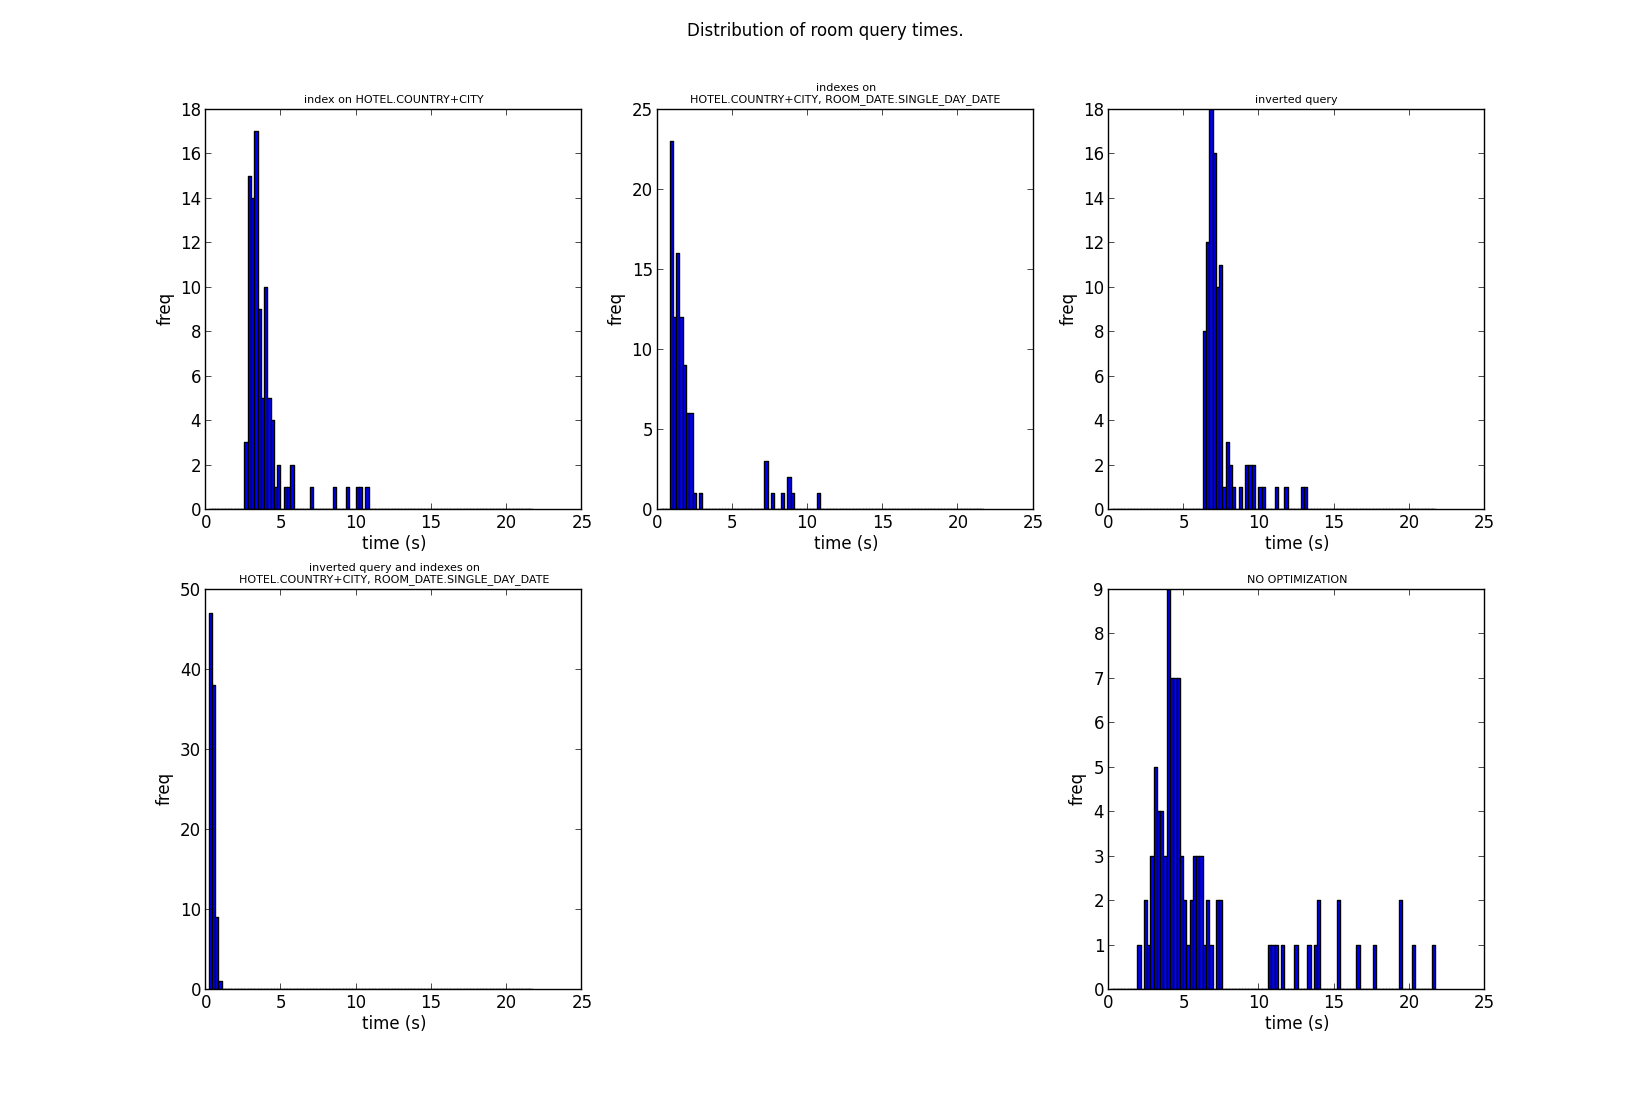
\includegraphics[width=\textwidth]{../ReserveWithUsApp/benchmark_data/1.png}
  \caption{Distribution of room query response times. Each plot corresponds to
    performance data collected after applying some subset of the proposed
    optimizations.}
  \label{fig:roomqueries}
\end{figure}

Looking at the format of the room query makes clear that the bulk of the
processing time is spent finding contiguous ranges of available
\texttt{SINGLE\_DAY\_DATE} entries and summing the room prices. We proposed a
clustered index on \texttt{SINGLE\_DAY\_DATE} to allow efficient scans of hotel
inventory for a specified date range.

One issue with indexing rooms is the frequency and contents of table updates.
Even if we update inventory on an hourly basis, it is likely that we can find a
setting for the proportion \texttt{PCTFREE} of table pages to leave enough free
space in order to avoid excessive overflow pages during inserts. The correct
setting of this parameter would either eliminate or diminish the need for
costly table reorganizations. We expect that updates should advance more or
less forward in time allowing the table to extend to new dates as sales staff
purchase inventory for upcoming dates.

We create the index by running the following commands:
\begin{Verbatim}[frame=single]
$ db2 CREATE INDEX ROOM_BY_DATE ON ROOM_DATE (SINGLE_DAY_DATE ASC) CLUSTER PCTFR
EE 10 COLLECT SAMPLED DETAILED STATISTICS
DB20000I  The SQL command completed successfully.
$ db2 RUNSTATS ON TABLE ROOM_DATE AND SAMPLED DETAILED INDEXES ALL
DB20000I  The RUNSTATS command completed successfully.
$ db2 REORG TABLE ROOM_DATE INDEX ROOM_BY_DATE ALLOW NO ACCESS INDEXSCAN
DB20000I  The REORG command completed successfully.
\end{Verbatim}
We can confirm the reorganization of the table data using the \texttt{db2pd}
utility:
\begin{Verbatim}[frame=single]
$ db2pd -db tuning -reorg
Database Member 0 -- Database TUNING -- Active -- Up 0 days 00:04:44 -- Date
2013-11-11-03.22.54.151273

Table Reorg Information:
Address            TbspaceID TableID PartID MasterTbs MasterTab TableName
Type    IndexID    TempSpaceID
0x00007F5F7D583EF8 2         4       n/a    n/a       n/a       HOTEL
Offline 2          2
0x00007F5F7D57FE78 2         6       n/a    n/a       n/a       ROOM_DATE
Offline 2          2

Table Reorg Stats:
Address            TableName          Start               End
PhaseStart          MaxPhase   Phase      CurCount   MaxCount   Status
Completion
0x00007F5F7D583EF8 HOTEL              11/11/2013 03:22:12 11/11/2013 03:22:17
11/11/2013 03:22:15 3          IdxRecreat 0          0          Done    0
0x00007F5F7D57FE78 ROOM_DATE          11/11/2013 03:18:16 11/11/2013 03:20:37
11/11/2013 03:19:00 3          IdxRecreat 0          0          Done    0
\end{Verbatim}
In this case, the table reorganization takes only a few minutes.

At this point, we observe in the results of Figure~\ref{fig:hotelqueries} show
that there is no significant difference between the results for hotel queries
with or without the indexes. As discussed already, this is likely due to the
small number of hotel rows.

The results in Figure~\ref{fig:roomqueries} for room queries show a nearly
$2\times$ gain over the hotel index alone by pushing the median response time
down to around 1.45s from 3.45s. The 99th percentile of queries went from
10.34s down to 9.07s.

\subsubsection{Inverting the room query}

By looking at the room query structure, we infer that a major and unnecessary
waste of computation lies in attempting to sum all hotels that satisfy the
target date range without filtering by the other attributes of the hotel query
such as \texttt{(CITY, COUNTRY)}. Inverting the query structure involves first
finding the list of eligible hotels and then summing price over the target date
range to find hotels with contiguous availability.

The following test case demonstrates the impressive performance gains possible
by inverting the query:
\begin{Verbatim}[frame=single]
$ time db2 select h.hotel_id, q.room_type_id, q.total_price from hotel h,
room_type rde, \( select rda.room_type_id, sum\(rda.price\) as total_price from
room_date rda where rda.numavail \> 0 and rda.single_day_date \>=
\'2013-11-05\' and rda.single_day_date \< \'2013-11-09\' group by
rda.room_type_id having count\(*\) = 4 \) q where h.hotel_id = rde.hotel_id and
h.city = \'city10\' and h.country = \'country3\' and q.room_type_id =
rde.room_type_id

HOTEL_ID    ROOM_TYPE_ID TOTAL_PRICE
----------- ------------ ---------------------------------
      28636        17251                             1105.
      28636        26903                              957.
      28636       290787                              960.

  3 record(s) selected.


real    0m4.089s
user    0m0.032s
sys     0m0.040s

$ time db2 select rda.room_type_id, sum\(rda.price\) from room_date rda, \(
select rde.room_type_id from room_type rde, hotel h where h.hotel_id =
rde.hotel_id and h.country = \'country3\' and h.city = \'city10\' \) q where
rda.numavail \> 0 and rda.single_day_date \>= \'2013-11-05\' and
rda.single_day_date \< \'2013-11-09\' and rda.room_type_id = q.room_type_id
group by rda.room_type_id having count\(*\) = 4

ROOM_TYPE_ID 2
------------ ---------------------------------
       17251                             1105.
       26903                              957.
      290787                              960.

  3 record(s) selected.


real    0m0.188s
user    0m0.024s
sys     0m0.032s
\end{Verbatim}
The example goes from approximately 4s before to 0.2s after, a gain of
approximately $20\times$. Note that this tests includes the indexes. A patch
to the ReserveWithUsApp enables this feature and it is available
\href{%
https://github.com/blr246/adbs-reservewithus/commit/4662879ee3443dcf48e1a692aed957891edd8e8c%
}{here}.

Since the room query has nothing to do with hotel-only queries, we examine only
the response times in Figure~\ref{fig:roomqueries} for room queries. The final
result in the lower-left-hand corner is an impressive 443ms median response
time down from 4.57s initially. In addition, the wide variance has all but
vanished entirely with the 99th percentile of queries taking 868ms down from
over 20s.  This is definitely a satisfactory result since the room query has a
response time just under $4\times$ greater than the hotel query rather than
$18\times$ greater as it was initially.

One interesting note is that, prior to adding the indexes, the inversion of the
room query succeeds in reducing the variance in room query response time while
failing to reduce the median. The plot in the upper-right-hand corner of
Figure~\ref{fig:roomqueries} presents the result under the title ``inverted
query'', and it serves as further evidence that the indexes are a critical
piece of this tuning recipe. A likely explanation is that indexes enable
efficient scans of subsets of relevant hotel and room table rows.

\begin{figure}[h!]
  \centering
  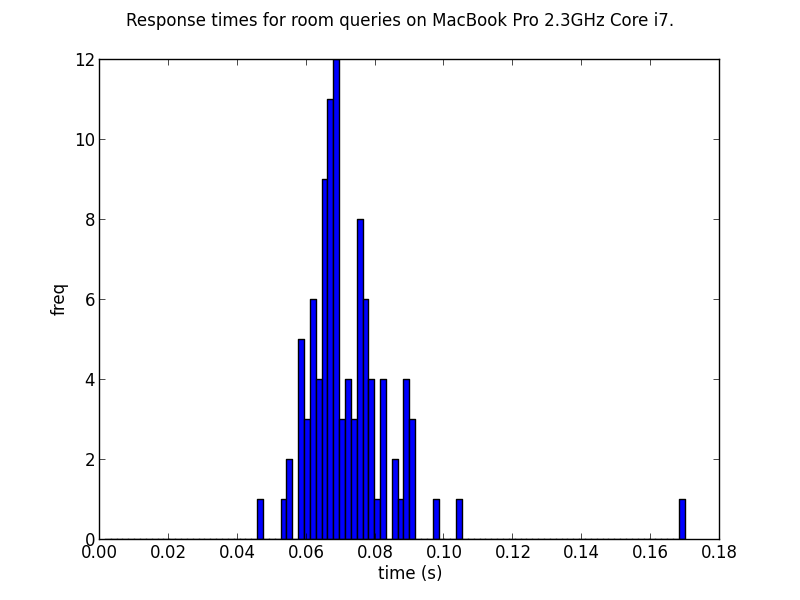
\includegraphics[width=0.5\textwidth]{../ReserveWithUsApp/benchmark_data/room_times_mbp.png}
  \caption{Distribution of room query response times.}
  \label{fig:roomqueriesmbp}
\end{figure}

An additional order of magnitude speedup is possible using modern hardware as
we see in Figure~\ref{fig:roomqueriesmbp}. The data are from a benchmark of
room queries run using the same virtual machine on a recent MacBook Pro with a
2.3GHz Intel Core i7 processor. The median response time for room queries is
around 69ms compared to 443ms for the weaker hardware, and the 99th percentile
of queries takes 98ms down from 868ms.

\subsection{Exporting and importing the customer table}

Exporting and importing an existing table is useful in the case when the
database system has been running for a while and so could benefit from
reorganizing the physical layout of the data on the storage media. A common
factor leading to performance degradations is the existence of overflow pages
since they decrease index performance. Reinitializing a table can give the
database system the opportunity to create a table using an optimal layout for
the data.

\subsubsection{Using \texttt{LOAD} and \texttt{EXPORT}}

One of the simplest mechanisms for exporting data is to write the table to disk
using the \texttt{EXPORT} command and then \texttt{LOAD} the saved data with a
\texttt{REPLACE} instruction that causes the database system to delete the
existing table and replace it.

The following is an example \texttt{EXPORT} operation on the \texttt{CUSTOMER}
table containing 1000000 rows.
\begin{Verbatim}[frame=single]
$ time db2 EXPORT TO customer.ixf OF IXF SELECT \* FROM CUSTOMER
SQL3132W  The character data in column "PASSWORD" will be truncated to size
"32700".

SQL3104N  The Export utility is beginning to export data to file
"customer.ixf".

SQL3105N  The Export utility has finished exporting "1000000" rows.


Number of rows exported: 1000000


real    0m52.824s
user    0m0.004s
sys 0m0.012s
\end{Verbatim}
Notice that we use the \texttt{IXF} output format because the binary data are
more efficient on disk than a human-readable format. This is important for
enabling faster export and import performance because there are fewer bytes to
read and write.

The following is an example \texttt{LOAD} operation on the \texttt{CUSTOMER}
table containing 1000000 rows.
\begin{Verbatim}[frame=single]
$ time db2 LOAD FROM customer.ixf OF IXF REPLACE INTO CUSTOMER
SQL3501W  The table space(s) in which the table resides will not be placed in
backup pending state since forward recovery is disabled for the database.

SQL3109N  The utility is beginning to load data from file
"/home/db2inst1/customer.ixf".

SQL3500W  The utility is beginning the "LOAD" phase at time "11/16/2013
14:41:54.111712".

SQL3150N  The H record in the PC/IXF file has product "DB2    02.00", date
"20131116", and time "133016".

SQL3153N  The T record in the PC/IXF file has name "customer.ixf", qualifier
"", and source "            ".

SQL3519W  Begin Load Consistency Point. Input record count = "0".

SQL3520W  Load Consistency Point was successful.

SQL3110N  The utility has completed processing.  "1000000" rows were read from
the input file.

SQL3519W  Begin Load Consistency Point. Input record count = "1000000".

SQL3520W  Load Consistency Point was successful.

SQL3515W  The utility has finished the "LOAD" phase at time "11/16/2013
14:41:57.183472".

SQL3500W  The utility is beginning the "BUILD" phase at time "11/16/2013
14:41:57.186797".

SQL3213I  The indexing mode is "REBUILD".

SQL3515W  The utility has finished the "BUILD" phase at time "11/16/2013
14:41:57.795943".


Number of rows read         = 1000000
Number of rows skipped      = 0
Number of rows loaded       = 1000000
Number of rows rejected     = 0
Number of rows deleted      = 0
Number of rows committed    = 1000000


real    0m3.868s
user    0m0.004s
sys 0m0.004s
\end{Verbatim}

The downsides to this approach are that
\begin{enumerate}[1.]
  \item the service or product must incur mandatory downtime in order to avoid
    data loss for records added after the \texttt{EXPORT} is initiated
  \item the \texttt{EXPORT} and \texttt{LOAD} operations incur heavy disk read
    and write costs and fail to make use of memory and shared resources within
    the core database system architecture
\end{enumerate}

\subsubsection{Using \texttt{REORG TABLE}}

The DB2 database system has a command called \texttt{REORG TABLE} that can
perform and in-place table reorganizing using internal database scratch space.
The procedure is similar to \texttt{EXPORT} and \texttt{LOAD REPLACE} except
that the operation does not require mandatory downtime, it can be paused and
resumed, it has a utility \texttt{REORGCHK} that verifies whether or not
reorganization is needed, and it uses optimizations internal to the database
system.

An example \texttt{REORGCHK} run follows.
\begin{Verbatim}[frame=single]
$ time db2 REORGCHK UPDATE STATISTICS ON TABLE CUSTOMER

Doing RUNSTATS ....


Table statistics:

F1: 100 * OVERFLOW / CARD < 5
F2: 100 * (Effective Space Utilization of Data Pages) > 70
F3: 100 * (Required Pages / Total Pages) > 80

SCHEMA.NAME                     CARD     OV     NP     FP ACTBLK    TSIZE  F1  F
2  F3 REORG
--------------------------------------------------------------------------------
--------
Table: DB2INST1.CUSTOMER
                             1000000      0  66703  66704      - 2.62e+08   0  9
7 100 ---
--------------------------------------------------------------------------------
--------

Index statistics:

F4: CLUSTERRATIO or normalized CLUSTERFACTOR > 80
F5: 100 * (Space used on leaf pages / Space available on non-empty leaf pages) >
MIN(50, (100 - PCTFREE))
F6: (100 - PCTFREE) * (Amount of space available in an index with one less level
/ Amount of space required for all keys) < 100
F7: 100 * (Number of pseudo-deleted RIDs / Total number of RIDs) < 20
F8: 100 * (Number of pseudo-empty leaf pages / Total number of leaf pages) < 20

SCHEMA.NAME                 INDCARD  LEAF ELEAF LVLS  NDEL    KEYS LEAF_RECSIZE 
NLEAF_RECSIZE LEAF_PAGE_OVERHEAD NLEAF_PAGE_OVERHEAD  PCT_PAGES_SAVED  F4  F5  F
6  F7  F8 REORG
--------------------------------------------------------------------------------
--------------------------------------------------------------------------------
---------------
Table: DB2INST1.CUSTOMER
Index: SYSIBM.SQL131111162740540
                            1000000  4167     0    3     0 1000000            4 
            4                710                 710                0   0  99   
3   0   0 *----
--------------------------------------------------------------------------------
--------------------------------------------------------------------------------
---------------

CLUSTERRATIO or normalized CLUSTERFACTOR (F4) will indicate REORG is necessary
for indexes that are not in the same sequence as the base table. When multiple
indexes are defined on a table, one or more indexes may be flagged as needing
REORG.  Specify the most important index for REORG sequencing.

Tables defined using the ORGANIZE BY clause and the corresponding dimension
indexes have a '*' suffix to their names. The cardinality of a dimension index
is equal to the Active blocks statistic of the table.


real    0m2.559s
user    0m0.008s
sys 0m0.004s
\end{Verbatim}

Here we see that formulas \texttt{F1, F2, F3, F5, F6, F7, F8} were all within
bounds as indicated by the `\texttt{-}' characters whereas the formula
\texttt{F4} is out of bounds as indicated by the `\texttt{*}'. This case calls
for \texttt{INDEX} reorganization as per the DB2 documentation.

The following command performs \texttt{INDEX} reorganization on the
\texttt{CUSTOMER} table.
\begin{Verbatim}[frame=single]
$ time db2 REORG INDEXES ALL FOR TABLE CUSTOMER ALLOW WRITE ACCESS REBUILD
DB20000I  The REORG command completed successfully.

real    0m3.057s
user    0m0.000s
sys 0m0.012s
\end{Verbatim}

This mechanism offers all of the advantages of \texttt{EXPORT} and
\texttt{LOAD} in one integrated command that allows the option to maintain
read/write access with degraded performance if mandatory downtime is not
possible.

\subsubsection{Using table clones}

The most ideal method for exporting and importing the \texttt{CUSTOMER} table is
using the \texttt{ALTER TABLE ADD CLONE} command available only for DB2 on IBM
z/OS. This command is documented \href{%
  http://publib.boulder.ibm.com/infocenter/dzichelp/v2r2/index.jsp?topic=%2Fcom.ib%
  m.db2z10.doc.admin%2Fsrc%2Ftpc%2Fdb2z_createclonetable.htm%
}{here}, and it is not available under our current system configuration. The
\texttt{CLONE} feature pairs with the \texttt{EXCHANGE TABLE} command, also not
available, which performs an efficient swap operation between cloned tables.

\subsection{Optimizing checkout}

\end{document}

